\begin{center}
\textbf{
\MakeUppercase{Приложение А}\\
(обязательное)\\
Исходный код}
\end{center}
\addcontentsline{toc}{section}{Приложение А (обязательное) Исходный код}

\lstinputlisting{inc/src/result_listing.swift}

\newpage

\newcommand{\pra}{
\begin{center}
\textbf{
\MakeUppercase{Приложение Б}\\
(информационное)\\
Антиплагиат}
\end{center}
\addcontentsline{toc}{section}{Приложение Б (информационное) Антиплагиат}
}

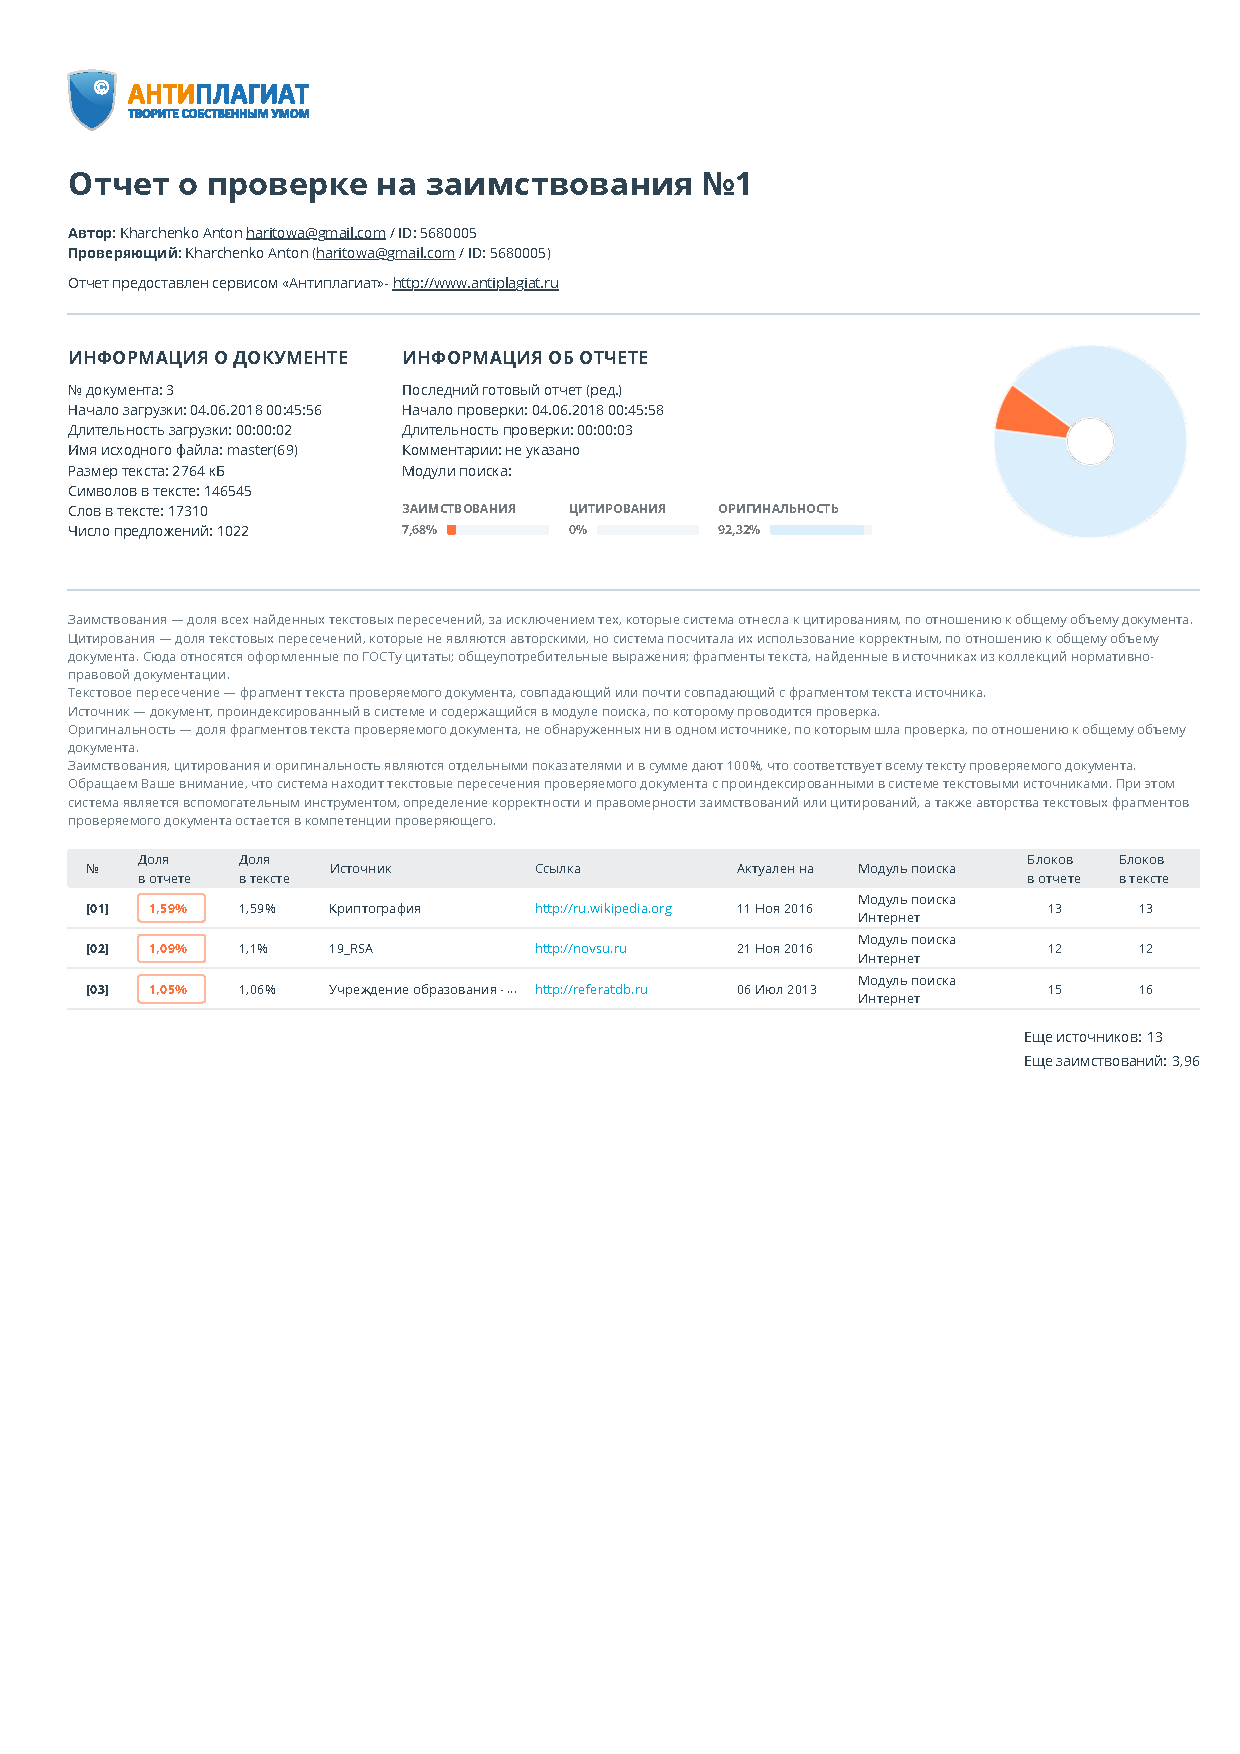
\includepdf[scale=0.8,pages=-,pagecommand={\pra}]{inc/pdf/antiplagiat.pdf}
\newpage


\begin{center}
\textbf{
\MakeUppercase{Приложение В}\\
(обязательное)\\
Ведомость документов}
\end{center}
\addcontentsline{toc}{section}{Приложение В (обязательное) Ведомость документов}

\newpage
\pagestyle{empty}
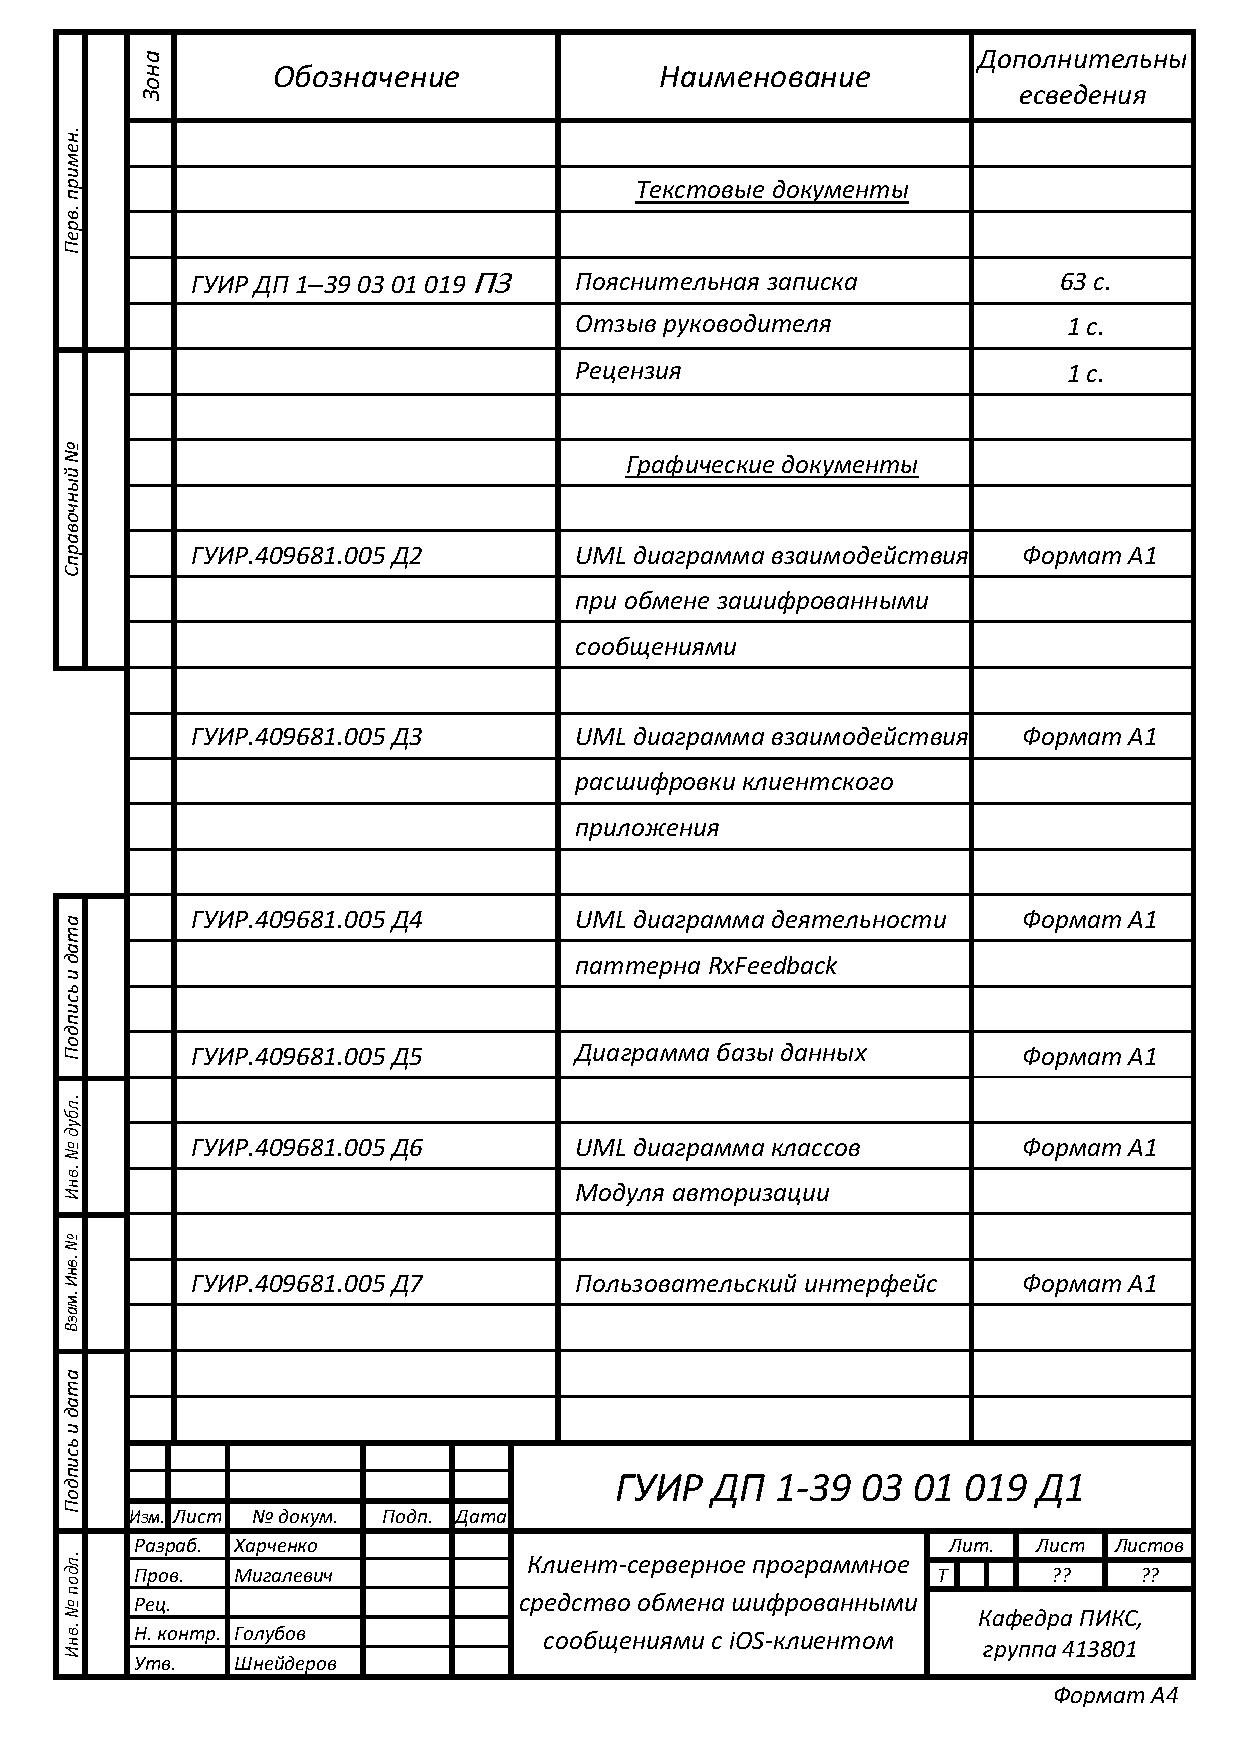
\includepdf[pages=-,pagecommand={}]{inc/pdf/vedomost.pdf}
\pagestyle{fancy}